%  LaTeX support: latex@mdpi.com 
%  For support, please attach all files needed for compiling as well as the log file, and specify your operating system, LaTeX version, and LaTeX editor.

%=================================================================
\documentclass[jrfm,article,submit,oneauthor,pdftex]{Definitions/mdpi} 
\usepackage{graphicx}
\usepackage{csvsimple,booktabs}

% For posting an early version of this manuscript as a preprint, you may use "preprints" as the journal and change "submit" to "accept". The document class line would be, e.g., \documentclass[preprints,article,accept,moreauthors,pdftex]{mdpi}. This is especially recommended for submission to arXiv, where line numbers should be removed before posting. For preprints.org, the editorial staff will make this change immediately prior to posting.

%--------------------
% Class Options:
%--------------------
%----------
% journal
%----------
% Choose between the following MDPI journals:
% acoustics, actuators, addictions, admsci, adolescents, aerospace, agriculture, agriengineering, agronomy, ai, algorithms, allergies, alloys, analytica, animals, antibiotics, antibodies, antioxidants, applbiosci, appliedchem, appliedmath, applmech, applmicrobiol, applnano, applsci, aquacj, architecture, arts, asc, asi, astronomy, atmosphere, atoms, audiolres, automation, axioms, bacteria, batteries, bdcc, behavsci, beverages, biochem, bioengineering, biologics, biology, biomass, biomechanics, biomed, biomedicines, biomedinformatics, biomimetics, biomolecules, biophysica, biosensors, biotech, birds, bloods, blsf, brainsci, breath, buildings, businesses, cancers, carbon, cardiogenetics, catalysts, cells, ceramics, challenges, chemengineering, chemistry, chemosensors, chemproc, children, chips, cimb, civileng, cleantechnol, climate, clinpract, clockssleep, cmd, coasts, coatings, colloids, colorants, commodities, compounds, computation, computers, condensedmatter, conservation, constrmater, cosmetics, covid, crops, cryptography, crystals, csmf, ctn, curroncol, currophthalmol, cyber, dairy, data, dentistry, dermato, dermatopathology, designs, diabetology, diagnostics, dietetics, digital, disabilities, diseases, diversity, dna, drones, dynamics, earth, ebj, ecologies, econometrics, economies, education, ejihpe, electricity, electrochem, electronicmat, electronics, encyclopedia, endocrines, energies, eng, engproc, ent, entomology, entropy, environments, environsciproc, epidemiologia, epigenomes, est, fermentation, fibers, fintech, fire, fishes, fluids, foods, forecasting, forensicsci, forests, foundations, fractalfract, fuels, futureinternet, futureparasites, futurepharmacol, futurephys, futuretransp, galaxies, games, gases, gastroent, gastrointestdisord, gels, genealogy, genes, geographies, geohazards, geomatics, geosciences, geotechnics, geriatrics, hazardousmatters, healthcare, hearts, hemato, heritage, highthroughput, histories, horticulturae, humanities, humans, hydrobiology, hydrogen, hydrology, hygiene, idr, ijerph, ijfs, ijgi, ijms, ijns, ijtm, ijtpp, immuno, informatics, information, infrastructures, inorganics, insects, instruments, inventions, iot, j, jal, jcdd, jcm, jcp, jcs, jdb, jeta, jfb, jfmk, jimaging, jintelligence, jlpea, jmmp, jmp, jmse, jne, jnt, jof, joitmc, jor, journalmedia, jox, jpm, jrfm, jsan, jtaer, jzbg, kidney, kidneydial, knowledge, land, languages, laws, life, liquids, literature, livers, logics, logistics, lubricants, lymphatics, machines, macromol, magnetism, magnetochemistry, make, marinedrugs, materials, materproc, mathematics, mca, measurements, medicina, medicines, medsci, membranes, merits, metabolites, metals, meteorology, methane, metrology, micro, microarrays, microbiolres, micromachines, microorganisms, microplastics, minerals, mining, modelling, molbank, molecules, mps, msf, mti, muscles, nanoenergyadv, nanomanufacturing, nanomaterials, ncrna, network, neuroglia, neurolint, neurosci, nitrogen, notspecified, nri, nursrep, nutraceuticals, nutrients, obesities, oceans, ohbm, onco, oncopathology, optics, oral, organics, organoids, osteology, oxygen, parasites, parasitologia, particles, pathogens, pathophysiology, pediatrrep, pharmaceuticals, pharmaceutics, pharmacoepidemiology, pharmacy, philosophies, photochem, photonics, phycology, physchem, physics, physiologia, plants, plasma, pollutants, polymers, polysaccharides, poultry, powders, preprints, proceedings, processes, prosthesis, proteomes, psf, psych, psychiatryint, psychoactives, publications, quantumrep, quaternary, qubs, radiation, reactions, recycling, regeneration, religions, remotesensing, reports, reprodmed, resources, rheumato, risks, robotics, ruminants, safety, sci, scipharm, seeds, sensors, separations, sexes, signals, sinusitis, skins, smartcities, sna, societies, socsci, software, soilsystems, solar, solids, sports, standards, stats, stresses, surfaces, surgeries, suschem, sustainability, symmetry, synbio, systems, taxonomy, technologies, telecom, test, textiles, thalassrep, thermo, tomography, tourismhosp, toxics, toxins, transplantology, transportation, traumacare, traumas, tropicalmed, universe, urbansci, uro, vaccines, vehicles, venereology, vetsci, vibration, viruses, vision, waste, water, wem, wevj, wind, women, world, youth, zoonoticdis 

%---------
% article
%---------
% The default type of manuscript is "article", but can be replaced by: 
% abstract, addendum, article, book, bookreview, briefreport, casereport, comment, commentary, communication, conferenceproceedings, correction, conferencereport, entry, expressionofconcern, extendedabstract, datadescriptor, editorial, essay, erratum, hypothesis, interestingimage, obituary, opinion, projectreport, reply, retraction, review, perspective, protocol, shortnote, studyprotocol, systematicreview, supfile, technicalnote, viewpoint, guidelines, registeredreport, tutorial
% supfile = supplementary materials

%----------
% submit
%----------
% The class option "submit" will be changed to "accept" by the Editorial Office when the paper is accepted. This will only make changes to the frontpage (e.g., the logo of the journal will get visible), the headings, and the copyright information. Also, line numbering will be removed. Journal info and pagination for accepted papers will also be assigned by the Editorial Office.

%------------------
% moreauthors
%------------------
% If there is only one author the class option oneauthor should be used. Otherwise use the class option moreauthors.

%---------
% pdftex
%---------
% The option pdftex is for use with pdfLaTeX. If eps figures are used, remove the option pdftex and use LaTeX and dvi2pdf.

%=================================================================
% MDPI internal commands
\firstpage{1} 
\makeatletter 
\setcounter{page}{\@firstpage} 
\makeatother
\pubvolume{1}
\issuenum{1}
\articlenumber{0}
\pubyear{2022}
\copyrightyear{2022}
%\externaleditor{Academic Editor: Firstname Lastname}
\datereceived{} 
%\daterevised{} % Only for the journal Acoustics
\dateaccepted{} 
\datepublished{} 
%\datecorrected{} % Corrected papers include a "Corrected: XXX" date in the original paper.
%\dateretracted{} % Corrected papers include a "Retracted: XXX" date in the original paper.
\hreflink{https://doi.org/} % If needed use \linebreak
%\doinum{}
%------------------------------------------------------------------
% The following line should be uncommented if the LaTeX file is uploaded to arXiv.org
%\pdfoutput=1

%=================================================================
% Add packages and commands here. The following packages are loaded in our class file: fontenc, inputenc, calc, indentfirst, fancyhdr, graphicx, epstopdf, lastpage, ifthen, lineno, float, amsmath, setspace, enumitem, mathpazo, booktabs, titlesec, etoolbox, tabto, xcolor, soul, multirow, microtype, tikz, totcount, changepage, attrib, upgreek, cleveref, amsthm, hyphenat, natbib, hyperref, footmisc, url, geometry, newfloat, caption

%=================================================================
%% Please use the following mathematics environments: Theorem, Lemma, Corollary, Proposition, Characterization, Property, Problem, Example, ExamplesandDefinitions, Hypothesis, Remark, Definition, Notation, Assumption
%% For proofs, please use the proof environment (the amsthm package is loaded by the MDPI class).

%=================================================================
% Full title of the paper (Capitalized)
\Title{Cap Rates as a Function of Real Economic Growth}

% MDPI internal command: Title for citation in the left column
\TitleCitation{Title}

% Author Orchid ID: enter ID or remove command
\newcommand{\orcidauthorA}{0000-0002-2151-468X} % Add \orcidA{} behind the author's name
%\newcommand{\orcidauthorB}{0000-0000-0000-000X} % Add \orcidB{} behind the author's name

% Authors, for the paper (add full first names)
\Author{Matthew Larriva, CFA$^{1,\dagger}$\orcidA{}}

%\longauthorlist{no}

% MDPI internal command: Authors, for metadata in PDF
\AuthorNames{Firstname Lastname, Firstname Lastname and Firstname Lastname}

% MDPI internal command: Authors, for citation in the left column
\AuthorCitation{Lastname, F.; Lastname, F.; Lastname, F.}
% If this is a Chicago style journal: Lastname, Firstname, Firstname Lastname, and Firstname Lastname.

% Affiliations / Addresses (Add [1] after \address if there is only one affiliation.)
\address[1]{%
$^{1}$ \quad FCP; mlarriva@fcpdc.com}

% Contact information of the corresponding author
\corres{Correspondence: e-mail@e-mail.com; Tel.: (optional; include country code; if there are multiple corresponding authors, add author initials) +xx-xxxx-xxx-xxxx (F.L.)}

% Current address and/or shared authorship
\firstnote{Current address: 4445 Willard Ave, Ste 900, Chevy Chase MD 20815} 
%\secondnote{These authors contributed equally to this work.}
% The commands \thirdnote{} till \eighthnote{} are available for further notes

%\simplesumm{} % Simple summary

%\conference{} % An extended version of a conference paper

% Abstract (Do not insert blank lines, i.e. \\) 
\abstract{This study investigates the interactive effect of changes in the Gross Domestic Product (GDP) and the Consumer Price Index (CPI) on US multifamily cap rates. The data from the US and 20 of its metropolitan statistical areas (MSAs) was used from 2000 to 2021. Accompanying cap rate data is sourced to Green Street. A binary logistic regression model was specified by reducing the interaction between first-differenced GDP and CPI to a single binary variable and reducing the first-differenced cap rate series to a binary variable. Cap rate changes are forecasted, and the model is evaluated using standard goodness of fit methods, a confusion matrix, and a comparison to a buy-and-hold strategy.  Overall, this study provides new evidence to explain and simplify the impact of inflation and economic growth on cap rates. The results show that the method of forecasting cap rates is highly robust in locations where growth is consistent with the national average (established cities) while it is less robust in fast-growing markets. It can be inferred that, in established cities and the US as a whole, cap rate growth can modelled as a function of only the underlying GDP growth relative to CPI growth.}

% Keywords
\keyword{Binary Logistic Regression; Cap Rates; US Real Estate Markets; Multifamily Cap Rate; Apartment Cap Rate} 

% The fields PACS, MSC, and JEL may be left empty or commented out if not applicable
%\PACS{J0101}
%\MSC{}
%\JEL{}

%%%%%%%%%%%%%%%%%%%%%%%%%%%%%%%%%%%%%%%%%%
% Only for the journal Diversity
%\LSID{\url{http://}}

%%%%%%%%%%%%%%%%%%%%%%%%%%%%%%%%%%%%%%%%%%
% Only for the journal Applied Sciences
%\featuredapplication{Authors are encouraged to provide a concise description of the specific application or a potential application of the work. This section is not mandatory.}
%%%%%%%%%%%%%%%%%%%%%%%%%%%%%%%%%%%%%%%%%%

%%%%%%%%%%%%%%%%%%%%%%%%%%%%%%%%%%%%%%%%%%
% Only for the journal Data
%\dataset{DOI number or link to the deposited data set if the data set is published separately. If the data set shall be published as a supplement to this paper, this field will be filled by the journal editors. In this case, please submit the data set as a supplement.}
%\datasetlicense{License under which the data set is made available (CC0, CC-BY, CC-BY-SA, CC-BY-NC, etc.)}

%%%%%%%%%%%%%%%%%%%%%%%%%%%%%%%%%%%%%%%%%%
% Only for the journal Toxins
%\keycontribution{The breakthroughs or highlights of the manuscript. Authors can write one or two sentences to describe the most important part of the paper.}

%%%%%%%%%%%%%%%%%%%%%%%%%%%%%%%%%%%%%%%%%%
% Only for the journal Encyclopedia
%\encyclopediadef{For entry manuscripts only: please provide a brief overview of the entry title instead of an abstract.}

%%%%%%%%%%%%%%%%%%%%%%%%%%%%%%%%%%%%%%%%%%
\begin{document}

%%%%%%%%%%%%%%%%%%%%%%%%%%%%%%%%%%%%%%%%%%

\section{Introduction}
The value of apartment stock in the US is 6 trillion dollars \citep*{nmhc},which constitutes over 1\% of the total wealth of the world \citep*{williams_2021}. Accurately projecting and explaining the value of that apartment stock has implications for direct investors, owners, renters, and anyone who owns part of the 255 billion dollars worth of securitized residential real estate that exists in public REITs \citep*{nareit_2022}. 

Despite the importance of explaining and forecasting the near and long-term value of this real estate, there is little to guide investors as to the direction of pricing, and therefore risk, of the asset class.

There has long been a supposed relationship between interest rates and cap rates\citep*{froland1987determines, sivitanides2001determinants, chandrashekaran2000predictability}. Supporters suggest that inflation rates are inversely related to cap rates either via real rates, the weighted average  cost of capital, or increased borrowing costs. More recent work suggests the relationship is not significant \citep*{larriva2021determinants}. 

To address periods where interest rates and cap rates deviate, models have introduced earnings expectations, demand-side factors, debt variables and spreads, and other variables. They often end with highly complex models that require regime-switching dynamics to account for the tail events (COVID-19, The Great Recession).

This study revisits the question of cap rate expansion from a simpler lens which treats cap rate compression as one binary outcome and cap rate expansion as the other, thus establishing a binary output variable. To explain the binary output variable, a binary input variable is used in a logistic regression. The input variable seeks to capture the dynamics of rent growth and expense growth through GDP growth and CPI growth, respectively. 

The remainder of the paper is outlined as follows: we review the literature surrounding cap rate forecasting and explanation as a function of GDP or growth metrics; CPI or inflationary metrics; or both variables together. Next we review the input data we used and the transformations we made. We then review our motivation for choosing a binary dependent variable and how we reduced the input variables to binary themselves. We specify a model and explain its validity by goodness of fit. The next section examines the results of our model, both at the national and MSA level. We review the results and show the strength of the model versus a buy-and-hold strategy before showing the cases (at the MSA-level) where the model works particularly well. Finally we conclude with suggestions for further research. 

\section{Literature Review}

The literature on cap rate forecasting is extensive, and it can be viewed well through two different lenses: variable selection and methodology selection. 

The first framework is illustrated in Ghysels et. al. Forecasting Real Estate Prices (\citeyear{ghysels_plazzi_valkanov_torous_2013}) which divides the literature by variable selection. The authors enumerate three camps: those models which use lagged return (or price change) as a variable, those which use ratios such as rent-to-price or price-to-income, and those which use more granular property or regional data. 

The second lens by which to view the research is through methodology selection, as documented by Larriva and Linneman (\citeyear{larriva2021determinants}). The authors divide the research into simple time series methods, multivariate timeseries, and machine learning methods. The division is roughly chronological. 

Neither lens quite suits this study's purpose, as the variables used in this work--raw GDP and CPI--are not often found in the research. More common is a spread to an inflation metric or a derivative of GDP. Separately, the level of granularity we seek to explain is somewhat uncommon (MSA level). More common is either property-level or national. Finally, the method we use is new to the research, to our review. The following section, then will seek to outline research that contains either growth or inflationary metrics, or their derivatives, regardless of method or granularity.

In the mid-1990s, research was concentrated on either single-variate autoregressive methods \citep*{gau_1984,gau_1985,linneman_1986} or variations on OLS that used multi-stage estimation \citep*{case_shiller_1990,abraham_hendershott_1994}. The variables used in these methods of forecasting tended to fall into classes that line up with the components of a cap rate: risk-free rate, real interest rates, relative return expectations, and risk. Many models’ variables included a government long-bond  to capture the risk-free and real rates, an economic spread (credit or pricing-based) to capture the relative expense or return of real estate, and macroeconomic factors to capture the  growth prospects and risk in the marketplace. Some models included a term to capture forward estimates including either sentiment or expected rent or NOI growth. This lines up with the Gordon growth model of pricing cap rates as the discount rate less the perpetual NOI growth rate. Thus, the value of macroeconomic factors, or their derivatives, was established.

\subsection{The Relationship between Inflation and Cap Rates}

Inflation has long been researched with regard to cap rates \citep*{froland1987determines, sivitanides2001determinants, chandrashekaran2000predictability}. Supporters suggest that inflation rates are inversely related to cap rates either via real rates, the weighted average  cost of capital, or increased borrowing costs. While there are myriad reasons why the relationship should hold, there are just as many observable exceptions--cases when cap rates increase when interest rates decline, or the reverse. Understandably then, the research into the topic reaches mixed conclusions.

\subsubsection{In Support of the Interest Rate and Cap Rate Relationship}
\cite{froland1987determines} reports negative correlations between cap rates and inflationary expectations. \cite{sivitanides2001determinants} further supported and quantified this relationship at the MSA level. The authors use the average cap rates over the past 16 years of four property types across 14 metropolitan markets to examine how cap rates behave. And the statistical specification was estimated using a dual Time-Series Cross-Section method which corrects for cross section correlations and group-wise heteroskedasticity. Inflation was found to be a major driver of cap rates. In fact, Sivitanides et al. found that an expected increase in economy wide inflation of one percent annually lowers office cap rates by 46 basis points, multi-family cap rates by 40 basis points, retail cap rates by 54 basis points, and by 20 basis points in industrial cap rates.

Research from \cite{wheaton2001real} further substantiates the above work using a VAR model to show that inflation is a significant variable in determining cap rates at the MSA level. 

\subsubsection{In Opposition of the Interest Rate and Cap Rate Relationship}
In contrast to the above works, \cite{chandrashekaran2000predictability} find that there is not a statistically significant relationship between inflation and cap rates. To reach this conclusion Chandrashekaran and Young use two regression models: one with macroeconomic variables and one with lagged cap rates. The model with lagged cap rates uniformly performed better. The authors concluded that their attempt to predict cap rates using macroeconomic variables, such as inflation, were unsuccessful. 

\cite{Gimpelevich2011} supports Chandrashekaran and Young using Monte Carlo simulations of real estate returns called the Simulation-Based Excess Return Model (SERM). The simulation results in poor correlation between inflation rates and cap rates.

More recently, \cite{larriva2021determinants} used multivariate timeseries analysis to show the superiority of a model which did not use return expectations or inflationary metrics. Their model used granger causality to select variables and establish a highly robust explanatory and predictive VECM model, without the use of interest rates.

Although there are exceptions, different conclusions in this space can often be attributed to differences in data and methodology. Research which finds that inflation is a good predictor of future cap rates typically use time series data for both macroeconomic variables and cap rates while research which dismisses the value of inflation rates, generally, use cross sectional econometric methods.

We propose herein that perhaps the reason for the disagreement in the impact of inflation rates to cap rates is because only some models are including the vital second part of the relationship: GDP.


\subsection{GDP}

The growth or contraction of a nation or MSA's gross domestic product is likely the single most important indicator of economic health. That cap rates would be closely related to this metric is not surprising. And there is ample research which substantiates and explores this.

Granger causality between GDP and real estate markets was established in 1997 by \cite{green1997follow} who found that, under a wide variety of time series specifications, residential investment causes GDP, while non-residential investment is caused by GDP. The phrase "caused by" is used in the Granger sense in this context. 

\cite{quan1997commercial} build on the Granger causality and seek to quantify the relationship. The team utilized time series regressions to examine the effects of changes in macroeconomic variables (including GDP) on real estate values and rents. To begin Quan and Titman explore the connection between stock and real estate market returns, and after establishing their connection the duo explore factors and develop regressions to explain this connection. The first theory they explore is that real estate and stock prices are both guided by future macroeconomic expectations such as GDP growth. The second is that commercial real estate prices rise and fall because of changing political and economic fundamentals, and under this theory the relationship between the stock and real estate market will be much weaker. After controlling for macroeconomic variance Quan and Titman find that the correlation between real estate and stock prices are primarily because of economic fundamentals, and that rental rates are strongly correlated with GDP growth.

Once this connection was established, research turned to its implication on an international scale: does worldwide GDP growth or local GDP growth have a larger effect on property values and cap rates? \cite{case2000global} explore whether or not correlations across global real estate markets are due to world changes in GDP, and estimate the value of local economic performance in real estate markets. This is an important question in real estate because all real estate is essentially local. And if local growth has a stronger effect on property values than national or global growth investors can better leverage local growth patterns to maximize return. The researchers found that that international property returns move together in dramatic fashion due to the effects of changes in GNP. Specifically, correlations of real estate are due in part to common exposure to fluctuations in the global economy, as measured by an equal-weighted index of international GDP changes. Some markets, such as Asia, are more effected by lo cal changes rather than world changes in GDP. In other words, even though real estate is fundamentally local changes in the global economy carry enough weight to have significant effects in local real estate markets.

\subsection{GDP and Inflation together}

Studies that focus on macroeconomic variables often include both GDP (or its derivative) and Inflation (or its derivative). The results often suggest that one variable is significant while the other is not. 

The aforementioned Quan and Titman research used cross sectional analyses to show that changes in GDP are very strongly related to movements in real estate values. But despite the significance of GDP, inflation and interest rates had relatively little effect on real estate values. Approaching the question with a timeseries analysis coroborated this conclusion. Quan and Titman found real estate values and rents were still significantly affected by changes in GDP. Inflation, again, appeared to be not significant. 

\cite{aizenman2009current} make a somewhat contrary finding. In their 2009 work, they determine that the most economically significant variable in accounting for changes in real estate valuation is lagged real estate valuation appreciation (defined as real estate inflation minus CPI inflation), followed in importance by lagged declines of Current Account divided by GDP. Thus they note that an inflation derivative is more important than a GDP derivative. 


\subsection{Current Methods}


In more recent years forecasting cap rates has embraced more advanced modeling techniques and more granular data.

Machine learning is well suited to forecasting cap rates as it is uniquely formulated to aggregate high parameter models, unlike many timeseries methods. Specifically, Random Forest models that consider a host of macroeconomic variables have been implemented to forecast future property values. The method allows the researcher to dismiss the hazards of autocorrelation of the input because the model does not assume uncorrelated residuals or independent input. As demonstrated by \cite{kok2017big}, the success is promising. 

\cite{christopoulos2020synthetic} employ Euclidian distancing to attempt to forecast cap rate series at the MSA level using unemployment and a house price index, but the study resorts to using regime switching mechanisms to fit to various cycles. While the forecasts generated are robust, the additional complexity from a regime switching model warrants caution in out-of-sample applications. 

The availability of more granular data, provided by large repositories of property financials, have made microeconomic approaches more available. \cite{li2020beyond} attempt to model cap rates based on a combination of property-specific and market-specific variables with success. 

Lastly, because the REIT markets have created a public market for real estate, there are analyses which seek to explain cap rates based on the faster pricing and higher liquidity offered by the equities markets. \cite{fisher2022location} illustrate a correlation between high-density locations and cap rates, corroborating the more microeconomic analysis of Li and Liang.


\subsection{Similar Models and Novelty}

The study that is most comparable to our own is that of \cite{duca2017taxes} whose research finds that cap rates are positively correlated with inflation via risk premia, and negatively correlated with rent growth expectations via GDP. Specifically, risk premia and real Treasury rates drive cap rates. They explain this theoretically via the discount factor (i.e. required rate of return).

Upon review, we note the frequency with which research disagrees on the significance (ordinal or absolute) of GDP metrics and inflation metrics. Our work makes three significant contributions to the existing body of work. 

First, we assert that neither GDP nor inflation variables are sufficient alone to explain cap rates. This can be seen by the above review. Simply using both as independent variables is not sufficient either. It is their interaction, we assert, that explains the most about cap rate directions. 

Second, we posit that we can learn more about cap rate determinants if we view cap rates as binary instead of continuous. While, of course, cap rate moves are non-discrete, this is not an useful way to analyze them, as real estate is still highly illiquid. The relevant question then, is not "will cap rates increase by, say,  0.0125 next year?" but instead "will cap rates increase next year?" Thus we model cap rate moves as random variables generated by a Bernouilli distribution as opposed to random variables generated by, say the Normal distribution. 

Finally, we propose a model that functions at the MSA and the national level. The more significant of these two is the former, because it determines the later. But the fact that the same data series are available at the nation and MSA and that they both corroborate the statistical findings is further attestation to the validity of the model.


\section{Materials and Methods}

\subsection{Data}
For the national model there are three data series that are used: the Consumer Price Index, the Gross Domestic Product, and the nominal Apartment cap rate series. 

\subsubsection{National}
The Gross Domestic Product is a quarterly, unadjusted (not de-seasoned) series from the St. Louis Fed's economic data page (FRED). It is important to use a nominal (versus real) series, as to not double count the impact of inflation, given the model takes into considration CPI changes separately.

The Consumer Price Index series is sourced to the Bureau of Labor Statistics, and it is also a non-seasonally adjusted series. In both cases, we did not seek to alter the series with seasonal adjustments because the raw data itself contains information which we do not wish to strip. Knowing if the economy grew faster than inflation, even if it was in 4Q, and even if it was due to holiday sales, is valuable information. Such a situation suggests a very different environment from its seasonally adjusted counterpart which may shows an economy in which 4Q growth is similar to say the prior quarter.

Finally, cap rate series at the national level are sourced to Green Street. Green Street defines its cap rate series as the next-twelve-months' NOI divided by the spot asset value. 

\subsubsection{Metropolitan}

MSA-level data follows the conventions of the national data. Non-seasonally adjusted series are selected both for MSA GDP and the MSA's CPI. The former is from FRED while the later is from the Bureau of Labor Statistics.

More challenging was the MSA-level data wherein GDP is presented only annually and CPI is presented with varying frequencies depending on the region. Atlanta is published on even months. Boston is published on odd months, and New York is published monthly. Some MSAs are published bimonthly. The Bureau of Labor statistics only offers CPI measures for 22 Core Based Statistical Areas (CBSA). Two of these are "Urban Alaska" and "Urban Hawaii", but these have no equivalent GDP series, so they were discarded. The remaining 20 CBSAs have GDP series. But the GDP series are not necessarily for the exact same areas i.e, some GDPs are published for an MSA, some are published for a CBSA. Adding to this confusion: the BLS revised its reporting in 2018 and started offering CBSA measurements instead of MSA measurements, thus revising the coverage areas.

To reconcile this, the study matches MSA to CBSA where needed (between the BLS and FRED). CPI measurements are averaged over a year before matching them to the GDP metrics. In this way, 21 geographies are produced for analysis: 20 MSAs and 1 national geography. Each geography has a cap rate, CPI, and GDP. 

As many practitioners assert that cap rates are functions of real interest rates, it is worth stating that the interaction effect between GDP and CPI, which we model, is not similar to real interest rates. Mathematically, the series have very low correlation. Practically, real rates contain an expectation of returns and an expectation of inflation, whereas GDP and CPI are merely spot empirical values.

Summary statistics are provided for each of the 20 MSAs as well as the national series in Table 1

\begin{table}[H] 
\caption{Average values of GDP (\$ 000s) CPI (unitless) and Cap Rates (\%) provided for each MSA as well as the national data: 2001-2021 \label{tab1}}
\csvautobooktabular{C:/Users/mlarriva/Documents/GitHub/inflation_cr_expansion/data/Average_Values.csv}
\end{table}



%%%%%%%%%%%%%%%%%%%%%%%%%%%%%%%%%%%%%%%%%%
\subsection{Model Construction}

\subsubsection{Model Selection}
While most analyses forecasting cap rates allow the random variable to be generated from a normal distribution, we opted instead to represent the variable as generated from a Bernoulli distribution. While this choice might be unorthodox--modelling a continuous variable as a binary variable-- we argue that it is well suited for two reasons. 

First, it is practical. Real estate is not an equity, it is an alternative asset. As such, it is illiquid. This lack of liquidity means an investor cannot enter and exit the market readily. As such, a would-be buyer is somewhat ambivalent between caring if a cap rate will go up by 40 basis points next year and if it  will simply go up. In either case, next year's prices will be lower. 

Second, it maps to the binary nature of the motivation of the model: will GDP growth (contraction) exceed CPI growth (contraction)? If so, then, ceteris paribus, tenants will be wealthier than the growth in expenses, and thus able to absorb higher rents, creating an asset worth more. Conversely, when inflation outpaces the growth of the economy, the tenant is not in a position to absorb higher costs, leaving the landlord to bear them, creating an asset worth less. 

Thus a logistic regression with a single binary input lent itself well to our analysis, with cap rate expansion as the response variable, and GDP change $ > $  CPI change as the independent variable. 

\subsubsection{Model Specification}

The GDP and CPI series were preprocessed differently for the national versus MSA model because the national data was more frequent. In both cases, the preprocessing included differencing the series and then creating a simple trailing average. The goal in smoothing the series was to prevent an overly sensitive signal. 

CPI and GDP percentage changes at $t_0$ were compared to trailing average historical percentage changes. A  signal was generated when 1) the $t_0$ GDP change was less than its trailing average changes and 2) the $t_0$ CPI change was greater than its trailing averages. The signal suggests cap rate expansion in the next period. 

The cap rate series were simply differenced and their sign taken to be a boolean variable such that cap rate expansion is TRUE and cap rate non-expansion (and contraction) is FALSE.

To establish the validity of the model for predictive power, we used a training and testing data set.

For the MSA model, five separate models were trained (Year = 2015, 2016....2020) which were specified using only data prior to that date. The each of the five models were used to predict the next years' (Years 2016-2021, 2017-2021,...2021) cap rate expansions and contractions based on the signal series outlined above. Each of these five models were specified as one--that is the data from each MSA was stacked into one matrix, absent the name of the MSA, and used to specify the model. The model then predicted the future values for each MSA based only on that MSA's historical data. Thus the same estimators were used to forecast the cap rate activity of the out-of-sample periods. Only the test data changed (was limited to only one MSA).

National models were created every two years from 2000, as data is both more frequent and longer lived than MSA-level data. 

Then, to establish the validity of the models for explanatory power, we trained both the MSA model and the national models using all time periods available (in-sample).

The ground truth of cap rate expansion does not present a balanced set, as cap rate compressions are far more frequent than cap rate expansions (roughly two to three times more years see compressions than expansions). The risk in modelling an unbalanced set is the risk of converging to an useless model that always forecasts the more common occurrence (i.e., always forecasting cap rate compression independent of the input). We overcame the imbalance through a Synthetic Minority Over-sampling Technique as created by \citep*{SMOTE}. This balanced the frequency of cap rate expansions and contractions to prevent a the logistic regression from estimating all compressions (which would produce a low-variance high-bias estimator).

\pagebreak

Thus our model can intuitively be understood in terms of the GDP and CPI historical series
\begin{equation}
GDP = \{g_i\}_{i=0}^N 
\end{equation}
\begin{equation}
CPI = \{c_i\}_{i=0}^N 
\end{equation}

...where $g_i$ and $c_i$ are the GDP and CPI values, respectively.
heir differenced series can be represented as
\begin{equation}
GDP' = \{g_i-g_{i-1}\}_{i=1}^N 
\end{equation}
\begin{equation}
CPI' = \{c_i-c_{i-1}\}_{i=1}^N 
\end{equation}

...and their respective n-period trailing averages, $h_i$ and $d_i$, are given by 
\begin{equation}
h_i=\frac{1}{n} \sum_{j=i-n}^{i}GDP'_j
\end{equation}
\begin{equation}
d_i=\frac{1}{n} \sum_{j=i-n}^{i}CPI'_j
\end{equation}

...such that comparing the current delta to prior averages determines cap rate expansion in the following way
\begin{equation}
  Cap\: Rate\:Expansion\:Variable_{t_i+1} =
  \begin{cases}
    0 & \text{if $GDP'_i-h_i > CPI'_i-d_i $} \\
    1 & \text{if $GDP'_i-h_i < CPI'_i-d_i $} \\
  \end{cases}
\end{equation}

Where 

\begin{equation}
  Cap\:Rate\:Expansion \sim \mathcal{B}(n=1,p=0.77)  
\end{equation}

And $p$ is given by the solution (coefficient) of the logistic regression:

\begin{equation}
p=\frac{1}{1+e^{(-\beta_1)(CRE variable)}}
\end{equation}

\begin{equation}
p=\frac{1}{1+e^{(-1.25)(1)}}
\end{equation}

\begin{equation}
p \approx 0.77
\end{equation}

The national model is specified by the following parameters:

\begin{equation}
Cap\:Rate\:Expansion_{t+8quarters} =  \frac{1}{1+e^{(-1.25)(CRE variable)}}
\end{equation}

where $h_i$ is solved for with $n=5$ and $d_i$ is solved for with $n=2$

The MSA model is specified by the following parameters:

\begin{equation}
Cap\:Rate\:Expansion_{t+1year} =  \frac{1}{1+e^{(-0.77)(CRE variable)}}
\end{equation}

where $h_i$ is solved for with $n=4$ and $d_i$ is solved for with $n=1$ and is backshifted 4

\subsubsection{Model Goodness of Fit}

In both the National and the MSA models, the logistic regressions displayed consistent coefficients, inline with our hypothesis. The coefficients had low standard errors relative  to the coefficients' magnitude, and the 2.5\% to 97.5\% bounds did not include zero in any case. 

Where a year is listed in the OOS in Year column, the data was segmented into training and test sets. The training periods were all prior to the split year, and the test set was the split year through 2021. When "all-time" is listed under the Split-Year, the model was trained on all data and evaluated on all avalailable data. 

The columns, "Coef.", "Std.Err.", "Z", "$P>|z|$", and the 2.5\% to 97.5\% bounds are all populated with the parameters from the trained models using the training data. The columns to the right, "accuracy" through "specificity" are based on the test data. 

It is worth noting that the coefficient decreased consistently as time advances, suggesting that perhaps the signal is not as robust as it once was. However the standard error decreases correspondingly, producing a Z score which is as high as the earlier periods. The decrease in the coefficient (corresponding to a lower probability of cap rate expansion for the CRE variable) could be due to the difficulty of trying to incorporate the GFC and the unorthodox interest rate behavior of the COVID-19 era. 

\begin{table}[H] 
\caption{Relevant parameters and metrics from the logistic regression trained on national data, both in and out of sample.\label{tab1}}
\csvautobooktabular{C:/Users/mlarriva/Documents/GitHub/inflation_cr_expansion/output/national_fit.csv}
\end{table}

\begin{table}[H] 
\caption{Relevant parameters and metrics from the logistic regression trained jointly on all MSA data, both in and out of sample.\label{tab1}}
\csvautobooktabular{C:/Users/mlarriva/Documents/GitHub/inflation_cr_expansion/output/msa_level_fit.csv}
\end{table}

\section{Results}

Upon implementing the models, results were evaluated using a confusion matrix, as the period we are attempting to capture--cap rate expansion-- is far less frequent than cap rate contraction. However, recall that  this was addressed by oversampling the data to produce a balanced set before specifying the models. To clarify, because cap rate expansion happens far less frequently than contraction, a naiive model could simply forecast constant cap rate compression, and it would be right a high percentage of the time. But this would not be useful for understanding cap rate determinants. To correct for this, a technique (referenced above as SMOTE) was used which balanced the number of cap rate compression and expansion periods by synthetically re-sampling the data. Thus our models would not suffer from biased overfitting.  

Accuracy (TP+TN/(TP+FP+TN+FN)) can be understood as the portion of time the model correctly identified a cap rate expansion or contraction. At the national level,cap rate expansion has happened 29.5\% of quarters since 2000. The national model, which was trained on data where cap rate expansions and compressions were equally frequent, is more accurate than a naiive model (forecasting constant cap rate compression), for all out-of-sample periods. At in-sample ('all-time') it is roughly as accurate as a naive model. This is not true at the MSA level, where cap rates have expanded 27\% of the time (compressed 73\% of the time) and the model yielded only 68\% accuracy. That is, it would have done better by forecasting constant cap rate compression (yielding an accuracy of 73\%). And, in contrast to the national  model, the MSA-level models perform better in-sample than out-of-sample.

Those subtleties are why it is necessary to examine precision, recall, and specificity. Precision (TP/(TP+FP)) is the ratio of correctly predicted positive observations to total predicted positive observations. The national model achieves 67\% precision, meaning two-thirds of the time a signal is generated, it is accurate. The jointly trained MSA model had relatively weak precision, out-of-sample, but surged to 68\% in-sample. 

Recall (TP/(TP+FN)) is the ratio of correctly identified cap rate expansions to the total number of cap rate expansions. In many MSAs there were only three or six years of cap rate expansions. Compare this to the national model which had far more quarters of cap rate expansion. The recall of the national model was high at 0.41, meaning 41\% of the times when cap rates expanded, the model correctly foretasted them. The recall of the MSA model was equal.

The F1-score combines the precision and recall into their harmonic mean, and is valuable to consider percision and recall together, though it is less intuitive. 

Finally, the specificity (TN/(TN+FN)) of both models was most noteworthy. A high specificity value suggests that the periods where cap rate compression was foretasted were highly accurate. This is especially useful in a series where cap rate compressions are profitable and are more common than expansions. These periods should not be missed, and indeed, the forecasts generated by both models would allow an investor to participate in upward of 80\% of the cap rate compressions experienced.

\begin{table}[H] 
\caption{A confusion matrix showing the values of the national model with both train/test split, and in-sample data.\label{tab1}}
\csvautobooktabular{C:/Users/mlarriva/Documents/GitHub/inflation_cr_expansion/output/national_accuracy.csv}
\end{table}

\begin{table}[H]
\caption{A confusion matrix showing the values of the MSA-level model with both train/test split, and in-sample data\label{tab1}}
\csvautobooktabular{C:/Users/mlarriva/Documents/GitHub/inflation_cr_expansion/output/msa_level_accuracy.csv}
\end{table}

Still, despite the four metrics of the confusion matrix, there remains the question of efficacy in practice. Because entering or exiting real estate holdings is not done easily or without great transactions costs, these models would only be useful to the extent they significantly outperformed a buy-and-hold strategy.

To examine this we implemented the national and MSA models' recommendations and yielded the following results.

\begin{figure}[H]
\includegraphics[scale=.9]{C:/Users/mlarriva/Documents/GitHub/inflation_cr_expansion/output/mas_graph_1_10.jpg}
\caption{The performance of the MSA-level forecasts versus a buy-and-hold strategy in each MSA, 1 through 10 of 20.\label{fig1}}
\end{figure}   
\unskip

\begin{figure}[H]
\includegraphics[scale=.9]{C:/Users/mlarriva/Documents/GitHub/inflation_cr_expansion/output/mas_graph_11_20.jpg}
\caption{The performance of the MSA-level forecasts versus a buy-and-hold strategy in each MSA, 11 through 20 of 20.\label{fig1}}
\end{figure}

\begin{figure}[H]
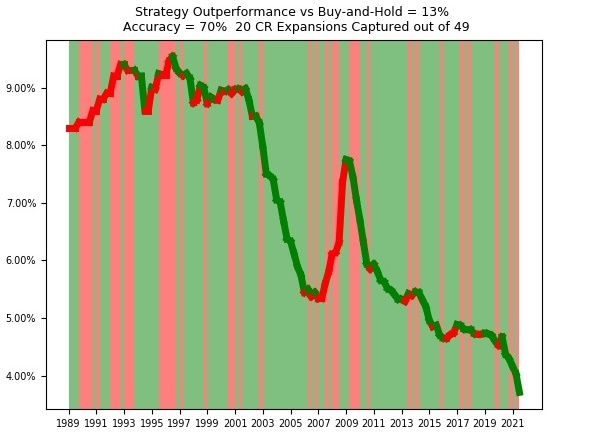
\includegraphics[scale=.9]{C:/Users/mlarriva/Documents/GitHub/inflation_cr_expansion/output/national_performance.jpg}
\caption{Graph of Forecast Performance at the National Level.\label{fig1}}
\end{figure}

At the national level, implementing the recommendations made by the model would have yielded cap rate compression 13\% greater than a buy-and-hold strategy. This would have happened in part because of the avoidance of sharp periods of cap rate expansion of the 2005-2009 period, and the late '80s.

At the MSA-level, implementing the recommendations would have resulted in significant outperformance of 29\% relative to a buy-and-hold strategy. But the variance is quite high. In Miami, implementing the model would have led to outperformance of 196\%, while in Baltimore, implementing the model would have resulted in underperformance of 66\%. Understanding these results is the  focus of the next section.

\pagebreak

\subsection{Analysis of Results}

The more robust predictor, in all cases, was the national model. This model, both in and out of sample, managed to forecast cap rate expansions accurately, with few false negatives and false positives. The model benefited from additional data points: both more history and more frequent readings. 

The MSA model that was jointly trained was relatively weak, which is likely owing to two factors. First, there is simply not enough data available. There were only 20 years of GDP and CPI data available consistently, and they were only reported annually. The model, however should not be disregarded, as data is becoming more widely distributed, with greater frequency, and with higher accuracy.

Upon further review, we noted that it seemed the MSAs wherein the model performed well were all established or low-population-growth cities, while the MSAs where the model performed poorly seemed to generally have higher population growth. 

Viewing these results in a regression, the results are more pronounced and show that household growth is significantly correlated with model underperformance, thus suggesting this model is very well suited for MSAs with national-average-like population growth. 

\begin{figure}[H]
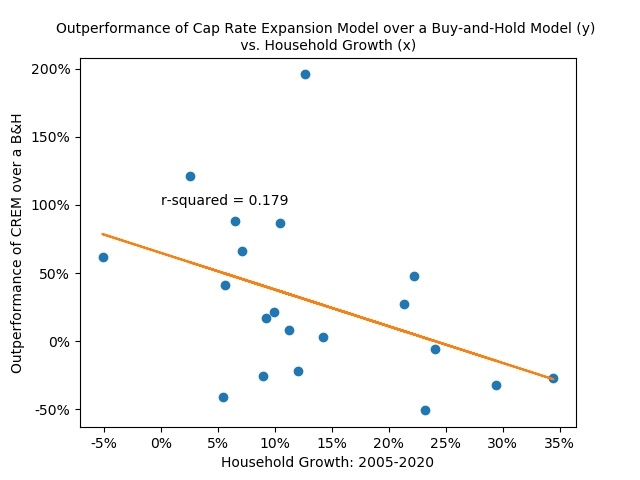
\includegraphics[scale=0.75]{C:/Users/mlarriva/Documents/GitHub/inflation_cr_expansion/output/msa_scatter.jpg}
\caption{The outperformance of the MSA-model over a buy-and-hold strategy versus the household growth of the MSA. Each dot represents one MSA. The X-axis shows the MSA's household growth over the model period while the Y-axis shows the outeprformance of the Cap Rate Expansion Mode. The graph illustrates that in MSAs (each dot) where household growth has been low, the strategy has outperformed \label{fig1}}
\end{figure}

\begin{table}[H]
\caption{The results of an ordinary least squares regression on the relationship between household growth and the outperformance of the cap rate model versus a buy-and-hold strategy.\label{tab1}}
\csvautobooktabular{C:/Users/mlarriva/Documents/GitHub/inflation_cr_expansion/output/ols_summary_all_msa.csv}
\end{table}

Removing the leverage point (Miami 196\% outperformance and 13\% household growth) yields an even tighter relationship.

\begin{figure}[H]
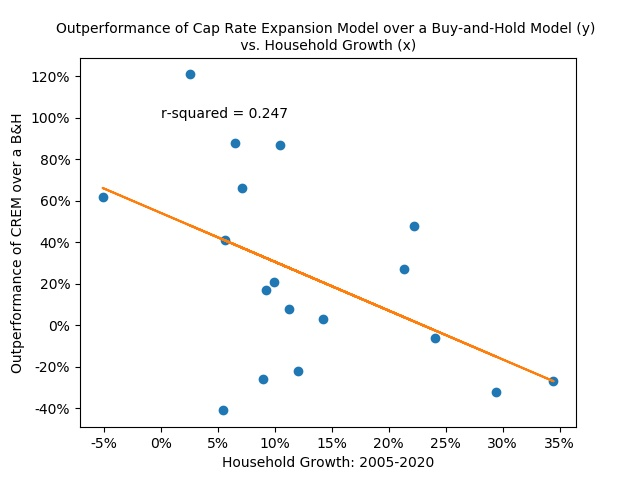
\includegraphics[scale=0.75]{C:/Users/mlarriva/Documents/GitHub/inflation_cr_expansion/output/msa_scatter_no_minmax.jpg}
\caption{The outperformance of the MSA-model over a buy-and-hold strategy versus the household growth of the MSA (leverage points removed). Each dot represents one MSA. The X-axis shows the MSA's household growth over the model period while the Y-axis shows the outeprformance of the Cap Rate Expansion Model. The graph illustrates that in MSAs (each dot) where household growth has been low, the strategy has outperformed \label{fig1}}
\end{figure}

\begin{table}[H]
\caption{The results of an ordinary least squares regression on the relationship between household growth and the outperformance of the cap rate model versus a buy-and-hold strategy. \label{tab1}}
\csvautobooktabular{C:/Users/mlarriva/Documents/GitHub/inflation_cr_expansion/output/ols_summary_all_msa_no_leverage.csv}
\end{table}

Relating the results to the original intent of the study: there are three salient findings.

First, modelling cap rate series and the independent variables as binary terms yielded statistically robust results. We argued that this binary viewing (cap rates either expanding or compressing) was nearly as telling as knowing the amount by which the rates would change, in a practical sense. And the model bore out that there was enough variance in the binary transformation to produce a robust analysis. This has implications for research in the cap rate sector in two areas: by simplifying cap rate models; by shedding light on the debate over the influence of real rates (vis-a-vis inflation) on cap rates.

Furthermore, the literature has debated the influence of interest rates on cap rates for some time. There seems to be no consistent conclusion. We suggest that the reason for the lack of consistency comes from the inclusion or exclusion of the GDP variable. That is, inflation and interest rates alone are not sufficient to forecast cap rates and can lead to inconsistent results. But the inclusion of the interaction term between GDP and CPI--or any growth versus real rates variable-- stabilizes this relationship.

Second, we use the interaction term to explain cap rate expansion and contraction at the national and MSA level, producing a robust confusion matrix with a strategy that outperforms buy-and-hold investing significantly. This has implications for all real estate investors at both the national and metropolitan levels, as all would benefit from clearer estimates of future values. MSA-level cap rate forecasting has been an undeserved area of research, yet it is the most relevant area for the research. Unlike public equities, a real estate investor would struggle greatly to own a nationally representative sample of properties. Instead, investors--even very large ones-- tend to focus in a handful of specific markets. Thus having higher confidence cap rate estimates within those markets is more relevant than knowing broad, quarterly, national cap rate forecasts.

Third, we address the high variance observed in the outperformance of our strategy versus a buy-and-hold strategy at the national level by relating it to household formation. As mentioned, implementing the forecasts generated by the model, at the MSA-level, produced outperformance on average. But there was a very high variance associated with this average, with the strategy outperforming by almost 200\% in some MSAs and by -61\% in others. One would be rightfully weary to implement this strategy on a new market. But upon further examination of these results, we confirmed that there existed a significant inverse relationship between average household formation and strategy outperformance. In markets where household formation were less-than-peer-group-average, the strategy outperformed, while in markets where household formation were greater-than-peer-group-average, the strategy underperformed. This has implications both for investors as well as for future research in the cap rate space. We suggest that future models not attempt to implement regime-switching techniques or any such advanced analytics, but instead to segment their data into markets of high growth and stable growth, knowing that the dynamics that govern cap rate movements in stable markets can easily be overridden by influxes of population. 


\section{Discussion}

The results have two main implications. The first is practical while the second is more academic. 

Practically, having an accurate forecast of cap rates at the MSA-level is valuable for property investors and owners. It allows a better understanding of what the future of the investment looks like. The results indicate that there is substantial outperformance to be had by investing based on the signals of the models as opposed to a buy-and-hold strategy--especially in stabilized markets. Conversely, in contexts where the model is less accurate--in high-growth markets-- it is valuable to know that the property markets can remain strong despite inflation and economic growth fluctuations.

Economically and at the national level, the model explains in what contexts real estate should be thought of as an inflationary hedge and in what contexts it will not hedge rising inflation. Investors often turn to real estate as a hard asset that will serve to maintain its value in rising interest rate environments. While that is sometimes true, this model assists in understanding when it is likely not true. 

More academically, the work serves as a potential explanation as to why there remains a disagreement in the impact of interest rates on cap rates. We posit that the reason some studies find interest rates important to real estate prices \citep{aizenman2009current}, is because in certain contexts they are very impactful (when they exceed GDP growth). And the reason other studies find interest rates to be not important to real estate values (\cite{quan1997commercial}, \cite{larriva2021determinants}) is because often times, they are not (when they are lower than GDP growth). Our model, in addition to showing when inflation is relevant to commercial real estate growth, simplifies the state of research which is trending toward more and more complex methodologies \citep{christopoulos2020synthetic} to explain a relationship which may be simpler than previously thought. 

\section{Conclusion}

In this study, we illustrated the efficacy of a simple logistic regression on forecasting and explaining cap rate expansion at the national and metropolitan-levels, with only a single input variable. This single input variable is a binary representation of the interaction between GDP and CPI changes relative to historical averages. Our theory in selection was that multifamily real estate depends mostly on an owner's ability to pass through inflation-like expenses to tenants. In cases where this is possible, the value of the property should increase.

We reduced cap rate movements to binary outcomes--expansions or contractions. And we reduced the independent variables to binary outcomes basically noting cases when GDP was expanding faster than CPI, relative to historical averages, respectively. We then specified a logistic regression model on data which had been resampled to produce a balanced set, avoiding the challenge created by cap rates which compress far more often than they expand. The models at the national and metropolitan levels were constructed both with rolling training and test sets and then again in-sample. All models were significant at a high threshold. 

When the recommendations of the models were implemented, there was significant outperformance versus a buy-and-hold strategy. But the outperformance of the MSA-level models was highly varied by metropolitan. We reexamined these results and noted the consistency of outperformance when an MSA was growing at a below-average rate. Based on this, we suggested that the dynamics which govern cap rate expansion vary in high-growth and low-growth markets. The latter is well explained by the binary model we produced, while the former was not. 

In those three ways, this research contributes to the existing body of work. It is the first, to our knowledge, work which analyses cap rates from a binary perspective rather than a continuous one. Second, the research adds to the few studies which have attempted to explain cap rates at a metropolitan level. And finally, it illustrates a more appropriate way to consider inflation and interest rates in the context of cap rate forecasting: by viewing them relative to growth instead of absolutely.

Areas for future research include broadening this analysis to more metropolitans. Data from the Bureau of Labor Statistics, which produces the Consumer Price Index, is not available consistently for other MSAs, but proxies are sure to be found. Similarly, testing an explicit wage variable may provide even further insight into cap rate expansion, beyond what is offered by the GDP variable. 

Given that the efforts to explain cap rates have become increasingly complex, and given the yet unsettled debate over the impact of inflation on real estate, this research offers a simplifying perspective. The question to be answered is not one of inflation versus disinflation, but one of relative inflation. This is independent from real rates, which have been another bogey in the cap rate forecaster's tool kit. Real rates contain expectations of future rates, while spot GDP and CPI series, used herein, are measures of current state. Real rates do not necessarily capture the growth in wages which tenants can afford to pay, while GDP changes come closer. 

Going forward, we encourage investors, owners, and anyone who participates in the multi-trillion dollar segment of American residential real estate to employ our analysis as an additional barometer of where real estate values may go. This may assist in reducing some of the confusion of investing and owning during the second or third once-in-a-lifetime financial event in which we find ourselves today.

\funding{This research was conducted as part of the professional role of the author as a researcher for a private equity firm.}

\informedconsent{Not applicable}

\dataavailability{Data and code available upon request} 

\acknowledgments{Walker Helvey assisted with data cleansing and literature review}

\conflictsofinterest{The author works for a private equity firm with real estate holdings throughout the US. The funders had no role in the design of the study; in the collection, analyses, or interpretation of data; in the writing of the manuscript; or in the decision to publish the~results.} 


\reftitle{References}

% Please provide either the correct journal abbreviation (e.g. according to the “List of Title Word Abbreviations” http://www.issn.org/services/online-services/access-to-the-ltwa/) or the full name of the journal.
% Citations and References in Supplementary files are permitted provided that they also appear in the reference list here. 

%=====================================
% References, variant A: external bibliography
%=====================================
\bibliography{bib}

%=====================================
% References, variant B: internal bibliography
%=====================================
%\begin{thebibliography}{999}
%% Reference 1
%\bibitem[Author1(year)]{ref-journal}
%Author~1, T. The title of the cited article. {\em Journal Abbreviation} {\bf 2008}, {\em 10}, 142--149.
%% Reference 2
%\bibitem[Author2(year)]{ref-book1}
%Author~2, L. The title of the cited contribution. In {\em The Book Title}; Editor 1, F., Editor 2, A., Eds.; Publishing House: City, Country, 2007; pp. 32--58.
%% Reference 3
%\bibitem[Author3(year)]{ref-book2}
%Author 1, A.; Author 2, B. \textit{Book Title}, 3rd ed.; Publisher: Publisher Location, Country, 2008; pp. 154--196.
%% Reference 4
%\bibitem[Author4(year)]{ref-unpublish}
%Author 1, A.B.; Author 2, C. Title of Unpublished Work. \textit{Abbreviated Journal Name} year, \textit{phrase indicating stage of publication (submitted; accepted; in press)}.
%% Reference 5
%\bibitem[Author5(year)]{ref-communication}
%Author 1, A.B. (University, City, State, Country); Author 2, C. (Institute, City, State, Country). Personal communication, 2012.
%% Reference 6
%\bibitem[Author6(year)]{ref-proceeding}
%Author 1, A.B.; Author 2, C.D.; Author 3, E.F. Title of presentation. In Proceedings of the Name of the Conference, Location of Conference, Country, Date of Conference (Day Month Year); Abstract Number (optional), Pagination (optional).
%% Reference 7
%\bibitem[Author7(year)]{ref-thesis}
%Author 1, A.B. Title of Thesis. Level of Thesis, Degree-Granting University, Location of University, Date of Completion.
%% Reference 8
%\bibitem[Author8(year)]{ref-url}
%Title of Site. Available online: URL (accessed on Day Month Year).
%\end{thebibliography}

% If authors have biography, please use the format below
%\section*{Short Biography of Authors}
%\bio
%{\raisebox{-0.35cm}{\includegraphics[width=3.5cm,height=5.3cm,clip,keepaspectratio]{Definitions/author1.pdf}}}
%{\textbf{Firstname Lastname} Biography of first author}
%
%\bio
%{\raisebox{-0.35cm}{\includegraphics[width=3.5cm,height=5.3cm,clip,keepaspectratio]{Definitions/author2.jpg}}}
%{\textbf{Firstname Lastname} Biography of second author}

% For the MDPI journals use author-date citation, please follow the formatting guidelines on http://www.mdpi.com/authors/references
% To cite two works by the same author: \citeauthor{ref-journal-1a} (\citeyear{ref-journal-1a}, \citeyear{ref-journal-1b}). This produces: Whittaker (1967, 1975)
% To cite two works by the same author with specific pages: \citeauthor{ref-journal-3a} (\citeyear{ref-journal-3a}, p. 328; \citeyear{ref-journal-3b}, p.475). This produces: Wong (1999, p. 328; 2000, p. 475)

%%%%%%%%%%%%%%%%%%%%%%%%%%%%%%%%%%%%%%%%%%
%% for journal Sci
%\reviewreports{\\
%Reviewer 1 comments and authors’ response\\
%Reviewer 2 comments and authors’ response\\
%Reviewer 3 comments and authors’ response
%}
%%%%%%%%%%%%%%%%%%%%%%%%%%%%%%%%%%%%%%%%%%
\end{adjustwidth}
\end{document}

